%\documentclass{standalone}
%\usepackage{tikz}
%\usetikzlibrary{patterns,plotmarks}
%\begin{document}
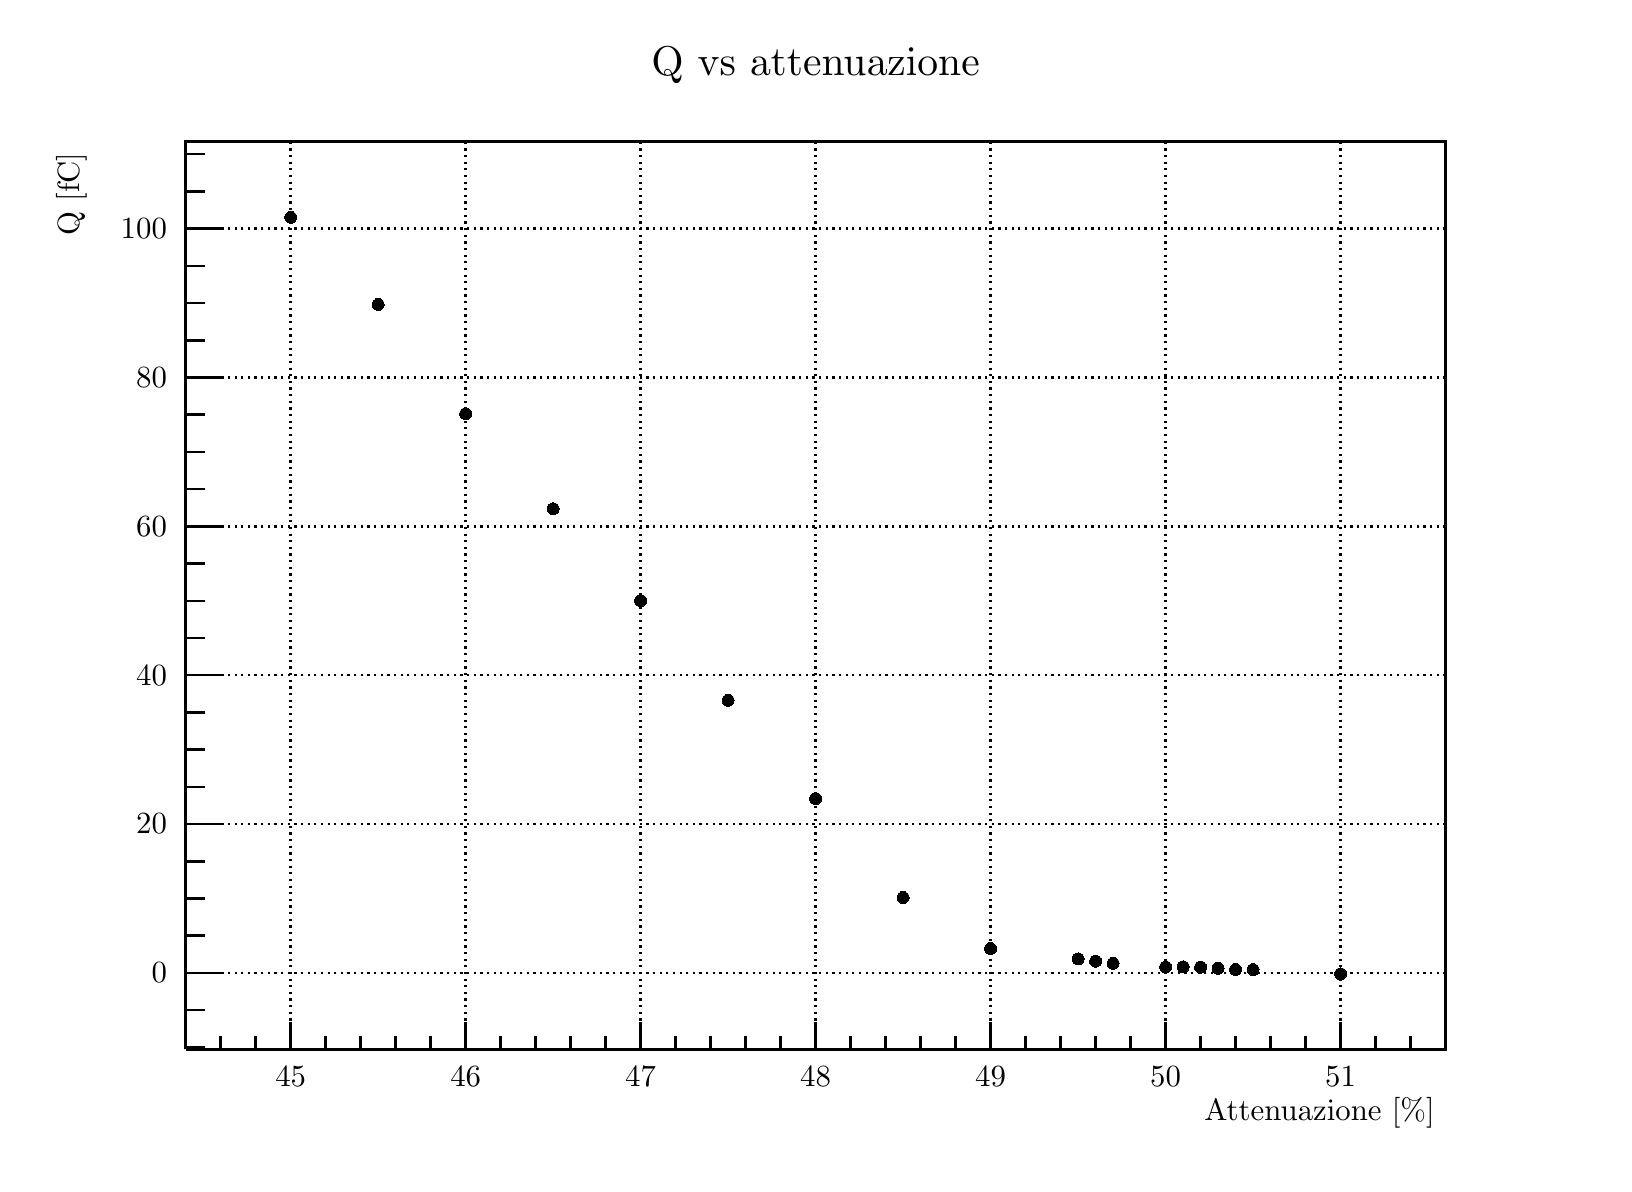
\begin{tikzpicture}
\def\CheckTikzLibraryLoaded#1{ \ifcsname tikz@library@#1@loaded\endcsname \else \PackageWarning{tikz}{usetikzlibrary{#1} is missing in the preamble.} \fi }
\CheckTikzLibraryLoaded{patterns}
\CheckTikzLibraryLoaded{plotmarks}
\pgfdeclareplotmark{cross} {
\pgfpathmoveto{\pgfpoint{-0.3\pgfplotmarksize}{\pgfplotmarksize}}
\pgfpathlineto{\pgfpoint{+0.3\pgfplotmarksize}{\pgfplotmarksize}}
\pgfpathlineto{\pgfpoint{+0.3\pgfplotmarksize}{0.3\pgfplotmarksize}}
\pgfpathlineto{\pgfpoint{+1\pgfplotmarksize}{0.3\pgfplotmarksize}}
\pgfpathlineto{\pgfpoint{+1\pgfplotmarksize}{-0.3\pgfplotmarksize}}
\pgfpathlineto{\pgfpoint{+0.3\pgfplotmarksize}{-0.3\pgfplotmarksize}}
\pgfpathlineto{\pgfpoint{+0.3\pgfplotmarksize}{-1.\pgfplotmarksize}}
\pgfpathlineto{\pgfpoint{-0.3\pgfplotmarksize}{-1.\pgfplotmarksize}}
\pgfpathlineto{\pgfpoint{-0.3\pgfplotmarksize}{-0.3\pgfplotmarksize}}
\pgfpathlineto{\pgfpoint{-1.\pgfplotmarksize}{-0.3\pgfplotmarksize}}
\pgfpathlineto{\pgfpoint{-1.\pgfplotmarksize}{0.3\pgfplotmarksize}}
\pgfpathlineto{\pgfpoint{-0.3\pgfplotmarksize}{0.3\pgfplotmarksize}}
\pgfpathclose
\pgfusepathqstroke
}
\pgfdeclareplotmark{cross*} {
\pgfpathmoveto{\pgfpoint{-0.3\pgfplotmarksize}{\pgfplotmarksize}}
\pgfpathlineto{\pgfpoint{+0.3\pgfplotmarksize}{\pgfplotmarksize}}
\pgfpathlineto{\pgfpoint{+0.3\pgfplotmarksize}{0.3\pgfplotmarksize}}
\pgfpathlineto{\pgfpoint{+1\pgfplotmarksize}{0.3\pgfplotmarksize}}
\pgfpathlineto{\pgfpoint{+1\pgfplotmarksize}{-0.3\pgfplotmarksize}}
\pgfpathlineto{\pgfpoint{+0.3\pgfplotmarksize}{-0.3\pgfplotmarksize}}
\pgfpathlineto{\pgfpoint{+0.3\pgfplotmarksize}{-1.\pgfplotmarksize}}
\pgfpathlineto{\pgfpoint{-0.3\pgfplotmarksize}{-1.\pgfplotmarksize}}
\pgfpathlineto{\pgfpoint{-0.3\pgfplotmarksize}{-0.3\pgfplotmarksize}}
\pgfpathlineto{\pgfpoint{-1.\pgfplotmarksize}{-0.3\pgfplotmarksize}}
\pgfpathlineto{\pgfpoint{-1.\pgfplotmarksize}{0.3\pgfplotmarksize}}
\pgfpathlineto{\pgfpoint{-0.3\pgfplotmarksize}{0.3\pgfplotmarksize}}
\pgfpathclose
\pgfusepathqfillstroke
}
\pgfdeclareplotmark{newstar} {
\pgfpathmoveto{\pgfqpoint{0pt}{\pgfplotmarksize}}
\pgfpathlineto{\pgfqpointpolar{44}{0.5\pgfplotmarksize}}
\pgfpathlineto{\pgfqpointpolar{18}{\pgfplotmarksize}}
\pgfpathlineto{\pgfqpointpolar{-20}{0.5\pgfplotmarksize}}
\pgfpathlineto{\pgfqpointpolar{-54}{\pgfplotmarksize}}
\pgfpathlineto{\pgfqpointpolar{-90}{0.5\pgfplotmarksize}}
\pgfpathlineto{\pgfqpointpolar{234}{\pgfplotmarksize}}
\pgfpathlineto{\pgfqpointpolar{198}{0.5\pgfplotmarksize}}
\pgfpathlineto{\pgfqpointpolar{162}{\pgfplotmarksize}}
\pgfpathlineto{\pgfqpointpolar{134}{0.5\pgfplotmarksize}}
\pgfpathclose
\pgfusepathqstroke
}
\pgfdeclareplotmark{newstar*} {
\pgfpathmoveto{\pgfqpoint{0pt}{\pgfplotmarksize}}
\pgfpathlineto{\pgfqpointpolar{44}{0.5\pgfplotmarksize}}
\pgfpathlineto{\pgfqpointpolar{18}{\pgfplotmarksize}}
\pgfpathlineto{\pgfqpointpolar{-20}{0.5\pgfplotmarksize}}
\pgfpathlineto{\pgfqpointpolar{-54}{\pgfplotmarksize}}
\pgfpathlineto{\pgfqpointpolar{-90}{0.5\pgfplotmarksize}}
\pgfpathlineto{\pgfqpointpolar{234}{\pgfplotmarksize}}
\pgfpathlineto{\pgfqpointpolar{198}{0.5\pgfplotmarksize}}
\pgfpathlineto{\pgfqpointpolar{162}{\pgfplotmarksize}}
\pgfpathlineto{\pgfqpointpolar{134}{0.5\pgfplotmarksize}}
\pgfpathclose
\pgfusepathqfillstroke
}
\definecolor{c}{rgb}{1,1,1};
\draw [color=c, fill=c] (0,0) rectangle (20,14.411);
\draw [color=c, fill=c] (2,1.4411) rectangle (18,12.9699);
\definecolor{c}{rgb}{0,0,0};
\draw [c,line width=0.9] (2,1.4411) -- (2,12.9699) -- (18,12.9699) -- (18,1.4411) -- (2,1.4411);
\definecolor{c}{rgb}{1,1,1};
\draw [color=c, fill=c] (2,1.4411) rectangle (18,12.9699);
\definecolor{c}{rgb}{0,0,0};
\draw [c,line width=0.9] (2,1.4411) -- (2,12.9699) -- (18,12.9699) -- (18,1.4411) -- (2,1.4411);
\draw [c,line width=0.9] (2,1.4411) -- (18,1.4411);
\draw [c,dash pattern=on 0.80pt off 1.60pt ,line width=0.9] (3.33333,12.9699) -- (3.33333,1.4411);
\draw [c,dash pattern=on 0.80pt off 1.60pt ,line width=0.9] (5.55556,12.9699) -- (5.55556,1.4411);
\draw [c,dash pattern=on 0.80pt off 1.60pt ,line width=0.9] (7.77778,12.9699) -- (7.77778,1.4411);
\draw [c,dash pattern=on 0.80pt off 1.60pt ,line width=0.9] (10,12.9699) -- (10,1.4411);
\draw [c,dash pattern=on 0.80pt off 1.60pt ,line width=0.9] (12.2222,12.9699) -- (12.2222,1.4411);
\draw [c,dash pattern=on 0.80pt off 1.60pt ,line width=0.9] (14.4444,12.9699) -- (14.4444,1.4411);
\draw [c,dash pattern=on 0.80pt off 1.60pt ,line width=0.9] (16.6667,12.9699) -- (16.6667,1.4411);
\draw [c,dash pattern=on 0.80pt off 1.60pt ,line width=0.9] (3.33333,12.9699) -- (3.33333,1.4411);
\draw [c,dash pattern=on 0.80pt off 1.60pt ,line width=0.9] (16.6667,12.9699) -- (16.6667,1.4411);
\draw [c,line width=0.9] (2,1.4411) -- (2,12.9699);
\draw [c,dash pattern=on 0.80pt off 1.60pt ,line width=0.9] (18,2.4133) -- (2,2.4133);
\draw [c,dash pattern=on 0.80pt off 1.60pt ,line width=0.9] (18,4.3038) -- (2,4.3038);
\draw [c,dash pattern=on 0.80pt off 1.60pt ,line width=0.9] (18,6.1943) -- (2,6.1943);
\draw [c,dash pattern=on 0.80pt off 1.60pt ,line width=0.9] (18,8.0848) -- (2,8.0848);
\draw [c,dash pattern=on 0.80pt off 1.60pt ,line width=0.9] (18,9.9753) -- (2,9.9753);
\draw [c,dash pattern=on 0.80pt off 1.60pt ,line width=0.9] (18,11.8658) -- (2,11.8658);
\draw [c,dash pattern=on 0.80pt off 1.60pt ,line width=0.9] (18,2.4133) -- (2,2.4133);
\draw [c,dash pattern=on 0.80pt off 1.60pt ,line width=0.9] (18,11.8658) -- (2,11.8658);
\draw [c,line width=0.9] (2,1.4411) -- (18,1.4411);
\draw [c,line width=0.9] (3.33333,1.78697) -- (3.33333,1.4411);
\draw [c,line width=0.9] (3.77778,1.61404) -- (3.77778,1.4411);
\draw [c,line width=0.9] (4.22222,1.61404) -- (4.22222,1.4411);
\draw [c,line width=0.9] (4.66667,1.61404) -- (4.66667,1.4411);
\draw [c,line width=0.9] (5.11111,1.61404) -- (5.11111,1.4411);
\draw [c,line width=0.9] (5.55556,1.78697) -- (5.55556,1.4411);
\draw [c,line width=0.9] (6,1.61404) -- (6,1.4411);
\draw [c,line width=0.9] (6.44444,1.61404) -- (6.44444,1.4411);
\draw [c,line width=0.9] (6.88889,1.61404) -- (6.88889,1.4411);
\draw [c,line width=0.9] (7.33333,1.61404) -- (7.33333,1.4411);
\draw [c,line width=0.9] (7.77778,1.78697) -- (7.77778,1.4411);
\draw [c,line width=0.9] (8.22222,1.61404) -- (8.22222,1.4411);
\draw [c,line width=0.9] (8.66667,1.61404) -- (8.66667,1.4411);
\draw [c,line width=0.9] (9.11111,1.61404) -- (9.11111,1.4411);
\draw [c,line width=0.9] (9.55556,1.61404) -- (9.55556,1.4411);
\draw [c,line width=0.9] (10,1.78697) -- (10,1.4411);
\draw [c,line width=0.9] (10.4444,1.61404) -- (10.4444,1.4411);
\draw [c,line width=0.9] (10.8889,1.61404) -- (10.8889,1.4411);
\draw [c,line width=0.9] (11.3333,1.61404) -- (11.3333,1.4411);
\draw [c,line width=0.9] (11.7778,1.61404) -- (11.7778,1.4411);
\draw [c,line width=0.9] (12.2222,1.78697) -- (12.2222,1.4411);
\draw [c,line width=0.9] (12.6667,1.61404) -- (12.6667,1.4411);
\draw [c,line width=0.9] (13.1111,1.61404) -- (13.1111,1.4411);
\draw [c,line width=0.9] (13.5556,1.61404) -- (13.5556,1.4411);
\draw [c,line width=0.9] (14,1.61404) -- (14,1.4411);
\draw [c,line width=0.9] (14.4444,1.78697) -- (14.4444,1.4411);
\draw [c,line width=0.9] (14.8889,1.61404) -- (14.8889,1.4411);
\draw [c,line width=0.9] (15.3333,1.61404) -- (15.3333,1.4411);
\draw [c,line width=0.9] (15.7778,1.61404) -- (15.7778,1.4411);
\draw [c,line width=0.9] (16.2222,1.61404) -- (16.2222,1.4411);
\draw [c,line width=0.9] (16.6667,1.78697) -- (16.6667,1.4411);
\draw [c,line width=0.9] (3.33333,1.78697) -- (3.33333,1.4411);
\draw [c,line width=0.9] (2.88889,1.61404) -- (2.88889,1.4411);
\draw [c,line width=0.9] (2.44444,1.61404) -- (2.44444,1.4411);
\draw [c,line width=0.9] (2,1.61404) -- (2,1.4411);
\draw [c,line width=0.9] (16.6667,1.78697) -- (16.6667,1.4411);
\draw [c,line width=0.9] (17.1111,1.61404) -- (17.1111,1.4411);
\draw [c,line width=0.9] (17.5556,1.61404) -- (17.5556,1.4411);
\draw [c,line width=0.9] (18,1.61404) -- (18,1.4411);
\draw [anchor=base] (3.33333,0.965539) node[scale=1.11327, color=c, rotate=0]{45};
\draw [anchor=base] (5.55556,0.965539) node[scale=1.11327, color=c, rotate=0]{46};
\draw [anchor=base] (7.77778,0.965539) node[scale=1.11327, color=c, rotate=0]{47};
\draw [anchor=base] (10,0.965539) node[scale=1.11327, color=c, rotate=0]{48};
\draw [anchor=base] (12.2222,0.965539) node[scale=1.11327, color=c, rotate=0]{49};
\draw [anchor=base] (14.4444,0.965539) node[scale=1.11327, color=c, rotate=0]{50};
\draw [anchor=base] (16.6667,0.965539) node[scale=1.11327, color=c, rotate=0]{51};
\draw [anchor= east] (18,0.634085) node[scale=1.11327, color=c, rotate=0]{Attenuazione [\%]};
\draw [c,line width=0.9] (2,1.4411) -- (2,12.9699);
\draw [c,line width=0.9] (2.48,2.4133) -- (2,2.4133);
\draw [c,line width=0.9] (2.24,2.88593) -- (2,2.88593);
\draw [c,line width=0.9] (2.24,3.35855) -- (2,3.35855);
\draw [c,line width=0.9] (2.24,3.83118) -- (2,3.83118);
\draw [c,line width=0.9] (2.48,4.3038) -- (2,4.3038);
\draw [c,line width=0.9] (2.24,4.77642) -- (2,4.77642);
\draw [c,line width=0.9] (2.24,5.24905) -- (2,5.24905);
\draw [c,line width=0.9] (2.24,5.72167) -- (2,5.72167);
\draw [c,line width=0.9] (2.48,6.1943) -- (2,6.1943);
\draw [c,line width=0.9] (2.24,6.66692) -- (2,6.66692);
\draw [c,line width=0.9] (2.24,7.13955) -- (2,7.13955);
\draw [c,line width=0.9] (2.24,7.61217) -- (2,7.61217);
\draw [c,line width=0.9] (2.48,8.0848) -- (2,8.0848);
\draw [c,line width=0.9] (2.24,8.55742) -- (2,8.55742);
\draw [c,line width=0.9] (2.24,9.03005) -- (2,9.03005);
\draw [c,line width=0.9] (2.24,9.50267) -- (2,9.50267);
\draw [c,line width=0.9] (2.48,9.9753) -- (2,9.9753);
\draw [c,line width=0.9] (2.24,10.4479) -- (2,10.4479);
\draw [c,line width=0.9] (2.24,10.9205) -- (2,10.9205);
\draw [c,line width=0.9] (2.24,11.3932) -- (2,11.3932);
\draw [c,line width=0.9] (2.48,11.8658) -- (2,11.8658);
\draw [c,line width=0.9] (2.48,2.4133) -- (2,2.4133);
\draw [c,line width=0.9] (2.24,1.94068) -- (2,1.94068);
\draw [c,line width=0.9] (2.24,1.46805) -- (2,1.46805);
\draw [c,line width=0.9] (2.48,11.8658) -- (2,11.8658);
\draw [c,line width=0.9] (2.24,12.3384) -- (2,12.3384);
\draw [c,line width=0.9] (2.24,12.811) -- (2,12.811);
\draw [anchor= east] (1.9,2.4133) node[scale=1.11327, color=c, rotate=0]{0};
\draw [anchor= east] (1.9,4.3038) node[scale=1.11327, color=c, rotate=0]{20};
\draw [anchor= east] (1.9,6.1943) node[scale=1.11327, color=c, rotate=0]{40};
\draw [anchor= east] (1.9,8.0848) node[scale=1.11327, color=c, rotate=0]{60};
\draw [anchor= east] (1.9,9.9753) node[scale=1.11327, color=c, rotate=0]{80};
\draw [anchor= east] (1.9,11.8658) node[scale=1.11327, color=c, rotate=0]{100};
\draw [anchor= east] (0.54812,12.9699) node[scale=1.11327, color=c, rotate=90]{Q [fC]};
\foreach \P in {(3.33333,12.0092), (4.44444,10.903), (5.55556,9.51534), (6.66667,8.30864), (7.77778,7.14216), (8.88889,5.87513), (10,4.6282), (11.1111,3.37122), (12.2222,2.72362), (13.3333,2.59089), (13.5556,2.56273), (13.7778,2.53458),
 (14.4444,2.48832), (14.6667,2.49033), (14.8889,2.48631), (15.1111,2.47223), (15.3333,2.45815), (15.5556,2.45614), (16.6667,2.40184)}{\draw[mark options={color=c,fill=c},mark size=2.162162pt, line width=0.000000pt, mark=*] plot coordinates {\P};}
\draw (10,13.9427) node[scale=1.50291, color=c, rotate=0]{Q vs attenuazione};
\end{tikzpicture}
%\end{document}
